\documentclass[a4paper,11pt]{article}
\usepackage[utf8]{inputenc}
\usepackage[russian]{babel}
\usepackage[T1]{fontenc}
\usepackage{amssymb,amsmath,graphicx,indentfirst}
\usepackage{caption}
\usepackage{color}
\usepackage{listings}
\usepackage{enumerate}
\usepackage[unicode]{hyperref}
\usepackage{qtree}
\usepackage{float}
\usepackage{epigraph}

\setlength{\parskip}{1ex plus 0.5ex minus 0.2ex}
\captionsetup[figure]{labelformat=empty}
\captionsetup[figure]{justification=centering}
\lstset{keywordstyle=\color{blue}\bfseries, basicstyle=\footnotesize}
\lstset{breaklines=true, breakatwhitespace=true}
\lstset{extendedchars=false, language=Caml, defaultdialect=[Objective]Caml}

\author{Олег Смирнов, Александр Полозов \\
\texttt{oleg.smirnov@gmail.com}, \texttt{polozov.alex@gmail.com}}
\date{2 декабря 2011 г.}
\title{Введение в функциональное программирование -- лабораторная работа \No 2}

\begin{document}
\epigraph{45\% of all Hadoop tutorials count words. 25\% count sentences.
20\% are about paragraphs. 10\% are log parsers. The remainder are 
helpful.}{@jandersen}

\section{Задача}
В индустрии часто возникают задачи, связанные с анализом данных, представленных
в виде графа. Одна из таких задач -- это поиск собственного вектора,
соответствующего наибольшему собственному числу матрицы смежности графа $A$.
Она лежит в основе алгоритмов ссылочного ранжирования страниц Интернет, 
алгоритма вычисления индекса цитируемости научых работ, ранжирования
пользователей социальных сетей и т.п.

Задача решается численно с помощью метода степенных итераций или его
разновидностей (степенной метод со сдвигом, с отсечением и др.) На первом шаге
метода выбирается начальное приближение -- вектор $\vec{x_0}$. На практике
можно просто взять единичный вектор.

На каждом $k$-м шаге алгоритм вычисляет $\vec{x_{k+1}} = 
\frac{A \vec{x_k}}{||A \vec{x_k}||}$. Можно показать, что метод сходится
со скоростью $|\frac{\lambda_2}{\lambda_1}|$, где $\lambda_1$ -- наибольшее
собственное число, а $\lambda_2$ -- следующее за ним.

В качестве критерия остановки алгоритма можно использовать, например,
следующий: $|\vec{x_{k+1}} - \vec{x_k}| < \epsilon$, где $\epsilon$ --
заданная точность.

\subsection{Параллелизация}
Для того, чтобы реализовать метод степенных итераций на больших объёмах
данных, необходима параллелизация вычислений. Технология MapReduce и
её открытая реализация Hadoop являются одним из наиболее удобных 
инструментов.

Задача программиста Hadoop -- представить алгоритм в виде пары функций:
\begin{itemize}
\item функцию $mapper$, которая преобразовывает входные пары ключ-значение
  в пары промежуточных результатов в том же формате:
  \begin{lstlisting}
    mapper (k1, v2) -> list<(k2, v2)>
  \end{lstlisting}
\item функцию $reducer$, которая получает пары из ключей и списков 
  промежуточных значений, соотвествующих этому ключу. Результатом функции
  должен быть список значений:
  \begin{lstlisting}
    reducer (k2, list<v2>) -> list<v3>
  \end{lstlisting}
\end{itemize}

\begin{figure}[h]
    \begin{center}
        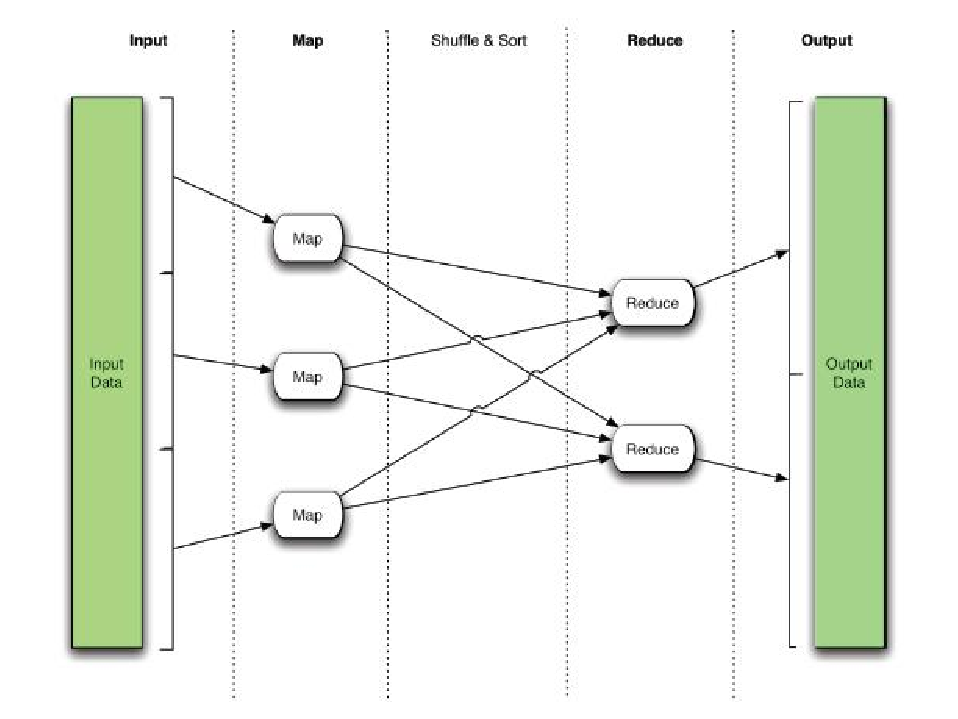
\includegraphics[height=100mm]{lab2/hadoop.eps}
        \caption{Этапы Hadoop}
    \end{center}
\end{figure}

Обработка данных на Hadoop состоит из последовательных этапов:
\begin{enumerate}
\item Input -- чтение исходных данных с распределённой файловой системы HDFS.
  На этом этапе пользователь может указать, как интерпретировать входную
  информацию. Hadoop поддерживает несколько стандартных форматов и позволяет
  определять собственные. Примеры форматов:
  \begin{enumerate}[(a)]
  \item $TextInputFormat$ -- данные в виде текстового файла. Ключ -- номер
    строки в файле, значение -- сама строка.
  \item $KeyValueTextInputFormat$ -- данные в виде текстового файла. Ключ --
    часть строки до символа-разделителя (обычно табуляция), значение --
    остальная часть строки.
  \end{enumerate}
\item Map -- обработка входных данных с помощью функции $mapper$.
\item Shuffle \& sort -- промежуточный этап между Map и Reduce. Данные
  перераспределяются между узлами кластера и группируются по значению
  промежуточного ключа.
\item Reduce -- обработка промежуточных данных с помощью функции $reducer$.
\item Output -- запись результатов на HDFS. Как и на этапе Input, пользователь
  может задавать формат сохранения результатов.
\end{enumerate}

``Родной'' язык Hadoop -- это Java. Однако система позволяет запускать
алгоритмы, реализованные на любых языках, с помощью интерфейса Streaming%
\footnote{\href{http://hadoop.apache.org/common/docs/current/streaming.html}
{http://hadoop.apache.org/common/docs/current/streaming.html}}.

Идея Streaming заключается в том, что Hadoop использует стандартный ввод/вывод
(stdin/stdout) для обмена данными с пользовательскими программами. 

\section{Задание}
\begin{enumerate}
\item Используя шаблоны $mapper.fs$ и $reducer.fs$ напишите решение для задачи
  подсчёта слов. В качестве тестового примера возьмите файл $lorem.txt$

  Для отладки решения можно использовать командную строку:
\begin{verbatim}
cat lorem.txt | mono mapper.exe | sort | mono reducer.exe
\end{verbatim}
\item Используя шаблоны, напишите алгоритм вычисления степенной итерации для
  поиска собственного вектора матрицы. В качестве входных данных возьмите файл 
  $ba\_100\_10.txt$. Файл описывает случайный граф из ста узлов, сгенерированный
  по модели Барабаси–Альберта в следующем формате:

  \begin{minipage}{0.49\linewidth}
    \Tree [.$0$ [.$1$ $2$ $3$ ] ]
  \end{minipage}
  \begin{minipage}{0.49\linewidth}
\begin{verbatim}
0    1
1    0 2 3
2    1
3    1 
\end{verbatim}
  \end{minipage}
  \begin{enumerate}[(a)]
  \item Проверьте вычисление одной итерации на локальной машине.
  \item Запустите вычисление на тестовом кластере Hadoop, взяв в качестве
    входных данных файл $ba\_40k\_120.txt$ -- случайный граф на 40000 узлов.
  \end{enumerate}
\item Напишите решение для задачи поиска десяти наиболее ``важных'' вершин в
  графе, используя в качестве меры важности ``eigenvector centrality''.
  
  Степенные итерации придётся вычислять последовательно, но каждую из итераций
  можно распараллелить. Для лабораторной достаточно вычислить фиксированное
  число итераций. На практике обычно используют связывание задач средствами
  Hadoop%
\footnote{\href{http://developer.yahoo.com/hadoop/tutorial/module4.html\#chaining}
{http://developer.yahoo.com/hadoop/tutorial/module4.html\#chaining}}.
  \begin{enumerate}[(a)]
  \item Проверьте вычисление одной итерации на локальной машине, взяв в
    качестве входных данных файл $ws\_100\_10.txt$ -- случайный граф из
    ста узлов по модели Воттса-Строгатца.
  \item Запустите вычисление на тестовом кластере на графе из 10000 узлов из
    файла $ws\_10k\_10.txt$.
  \end{enumerate}
\end{enumerate}
\end{document}
